% Chapter Template

\chapter{Secure Compartmentalisation} % Main chapter title

\label{Chapter 6} % Change X to a consecutive number; for referencing this chapter elsewhere, use \ref{ChapterX}

This chapter goes over the frame work for how secure compartments will be implemented in the MEGA65. It will then discuss the problems encountered during the implementation of the secure compartments. Finally this chapter will talk about the possible issues with the secure compartments.

%----------------------------------------------------------------------------------------
%	SECTION 1
%----------------------------------------------------------------------------------------

\section{Theorised Operation}

\label{Ch6 Sec1}

Thanks to the work of Tim Kirby, a frame work was provided for the operation of the secure compartments of the phone, as seen in figure \ref{fig:timkirby}. From this diagram, the finite state machine seen in figure \ref{fig:securecompartmentsfsm} was created and the state transition actions were noted. As seen in both figures \ref{fig:timkirby} and \ref{fig:securecompartmentsfsm}, initially the user begins in the insecure user mode. This user mode is then halted via a hypervisor trap that causes the io registers and the RAM and ROM of the phone to be saved to the SD card. The non-transfer section of RAM and all of ROM are then erased. From one of the save-state slots on the SD card, the desired secure service is then loaded into ROM. As soon as this is finished matrix mode is triggered and the CPU is halted. Matrix mode causes all external input into the phone, apart from the keyboard, to be cut off. At this point the user is able to inspect ROM and the transfer area of RAM. If the user is satisfied, by typing "ACCEPT" the secure service is then allowed to execute with the data provided in the transfer area of RAM. If the user is dissatisfied, by typing "REJECT" the secure service is erased from ROM, matrix mode is then left and the CPU is resumed. The hypervisor then uses the save-state created immediately prior to entering matrix mode to restore the io registers and load all the data that was saved back into RAM and ROM. If the secure container was accepted, any additional trap to the hypervisor will be seen as an exit request from the secure container. During an exit request, the user will once again be prompted to inspect the transfer area of RAM and then accept or reject the escaping of the of that data from the secure container. If satisfied, by typing "ACCEPT" the non-transfer section if RAM and all of ROM are once again erased. Then matrix mode is left and, identically to the user rejecting entry into the secure container, the CPU is resumed. The hypervisor then loads the save-state created immediately prior to entering matrix mode from the SD card, which is used to restore the io registers and reload data back into non-transfer RAM and ROM. If the user is dissatisfied with data escaping the secure container, by typing "REJECT" all of RAM and all of ROM are erased before the matrix mode exit. Then the save-state is loaded identically to the accepted exit case by the hypervisor and the resumed CPU. Finally, an exit status flag is raised depending on how the secure service transaction went.

\begin{figure}
  \centering
  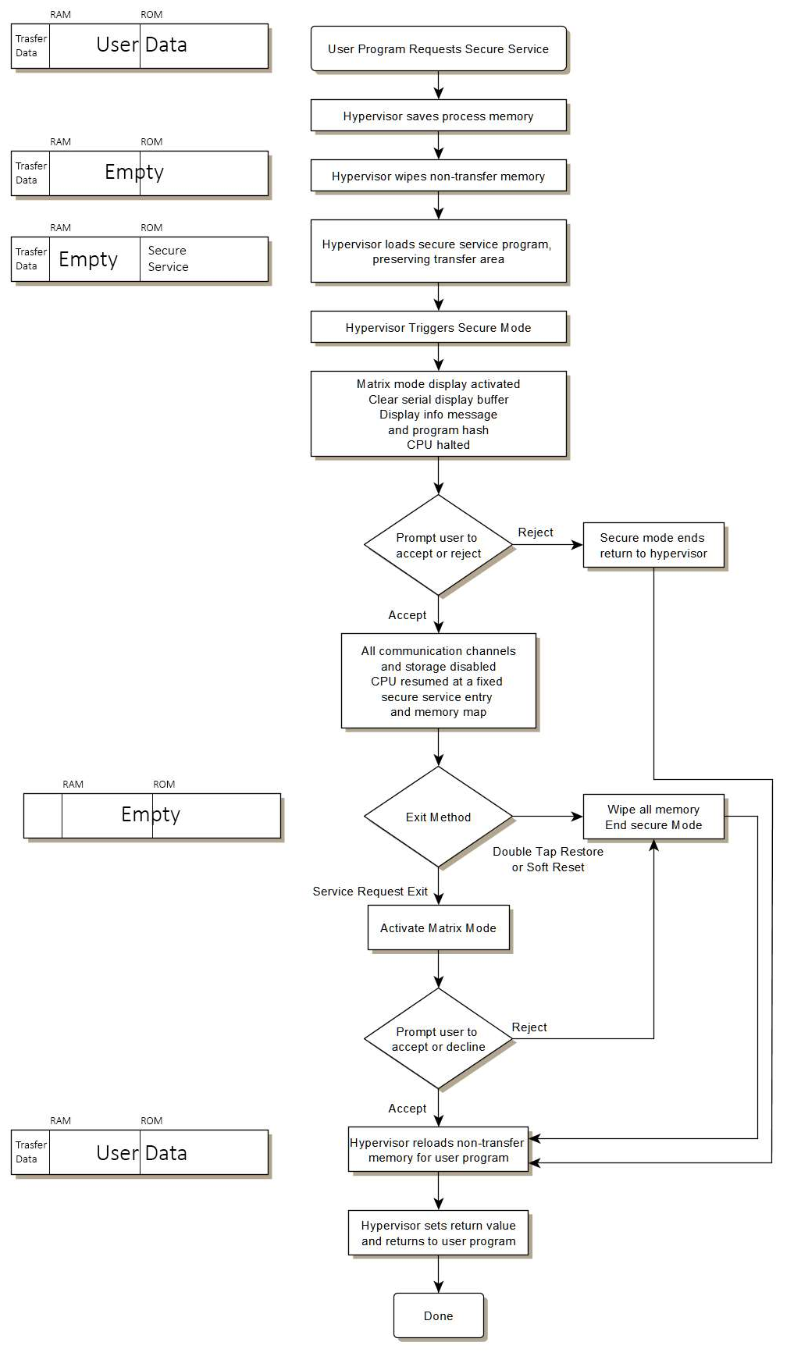
\includegraphics[width=\linewidth]{timkirby}
  \caption{The secure compartment frame work provided by Tim Kirby's thesis "Design and Development of a Secure Compartmentalised 8-bit Architecture".}
  \label{fig:timkirby}
\end{figure}

%----------------------------------------------------------------------------------------
%	SECTION 2
%----------------------------------------------------------------------------------------

\section{Initial Issues}

\label{Ch6 Sec2}

As the secure compartments were entirely separate from the matrix mode corrections and during the timea major update for another section of the phone was finished, a new branch of the project was created. Switching to this new branch resulted in overhead issues that needed to be solved in order for the project to procceed further.

%-----------------------------------
%	SUBSECTION 1
%-----------------------------------
\subsection{Repairing the Branch}

\label{Ch6 Sec2 Sub1}

As a new section of the project was being worked on the by other developers in isolation from the changes I had made, many of the fixes I had implemented had to be redone.\\
The timing fixes done to possibly correct the matrix mode issue were all removed, including the generation of the timing reports, these were reimplemented. The implementation was identical to that described in section \ref{Ch5 Sec1 Sub2} of chapter \ref{Chapter 5}.\\
All of the letterboxing changes were lost, so, as seen in section \ref{Ch5 Sec2} of chapter \ref{Chapter 5}, the erasing of the second character set was done one gains and the letterbox signal was one again used to limit the output of matrix mode.\\
The revolving line issue due to discrepancies in line length returned as was fixed as described in section \ref{Ch5 Sec3 Sub1} of chapter \ref{Chapter 5}.\\

In addition to the minor issues, matrix mode was not behaving as intended again. When attempting to enter or exit matrix mode with the tab + C= key combination, the key combination would be read and re-read rapidly and continuously. This made entering and exiting matrix mode unreliable as it was up to luck whether the key combination was scanned an odd or even amount of times to determine if the state was toggled. Tracing the matrix mode hypervisor trap from the CPU to the io mapper shows, as seen in figure \ref{fig:mmlatch}, there are latching and unlatching conditions for the matrix mode hypervisor trap. When monitoring the ascii\_key\_valid and ef\_latch signals via oscilloscope, the cause of the issue was clear. The ascii\_key\_valid signal was not a latching signal, and thus, it would only be high for a single clock cycle. As seen in the logic in figure \ref{fig:mmlatch}, this would cause the latch signal to pulse simillarly, allowing the matrix mode hyper trap to be triggered every second clock cycle. A quick solution to this issue, as seen in figure \ref{fig:traptimeout} was written by Dr. Gardner-Stephen in the form of a timeout clock that blocks repeated instances of tab + C= from triggering the matrix mode hypervisor trap.

\begin{figure}
  \centering
  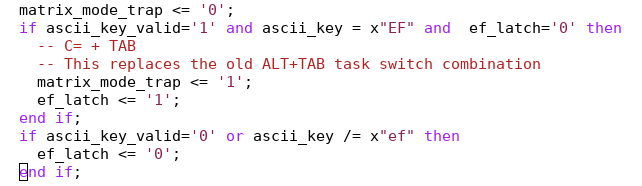
\includegraphics[width=\linewidth]{mmlatch}
  \caption{The matrix mode hypervisor trap latch.}
  \label{fig:mmlatch}
\end{figure}

\begin{figure}
  \centering
  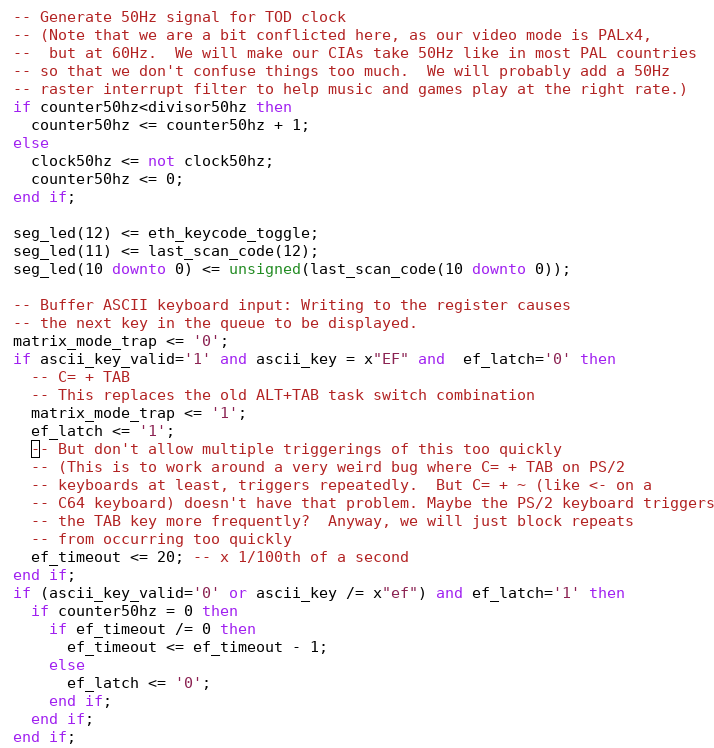
\includegraphics[width=\linewidth]{traptimeout}
  \caption{The matrix mode hypervisor trap latch with the new timeout period to prevent constant triggering.}
  \label{fig:traptimeout}
\end{figure}

%-----------------------------------
%	SUBSECTION 2
%-----------------------------------
\subsection{SD Card Restoration}

\label{Ch6 Sec2 Sub2}

One of the already implemented functions on the phone was the freeze function, this allowed the user to save state to a "Slot" located on the SD card. This freeze function would be the basis for the saving to and loading from the SD card when entering and exiting secure mode. The functionality for the standard capacity SD cards (SDSC) was entirely as expected, it was only the high capacity SD cards (SDHC) that were causing issues. When attemping to write to an SDHC card with the existing code, no visible errors occured. It was only when attemping to read from this card that an issue occured. When attemping to read after the first time the SD card would read no data, each read required a reset of the SD card between them in order for correct functionality. The extreme capacity SD card (SDXC) was not supported by the current hardware and indeed, was not recognised as an SD card at all when reading and writing was attempted. At the suggestion of Dr. Garner-Stephen, the issue with the SDHC cards was examined from the finite state machine located in the sdcard.vhdl file. As seen in figure \ref{fig:sdcardread} when reading or writing, the SD card is selected by making the cs\_bo bit low, and when it is not doing either of them, it is deselected by making cs\_bo high. Comparing this to the reset proccess seen in figures \ref{fig:resetsdcard}, \ref{fig:startsdcard} and \ref{fig:deselectsdcard}, it can be seen that there are several signals that are not being propogated when deselecting the SD card. At the suggestion of Dr. Gardner-Stephen, the simple solution of not deselecting the SD card was used. This solution, as seen in figure \ref{fig:sdcardfix}, does not provide hot swapping of the SD card, but has the functionality required for the secure mode implementation.

\begin{figure}
  \centering
  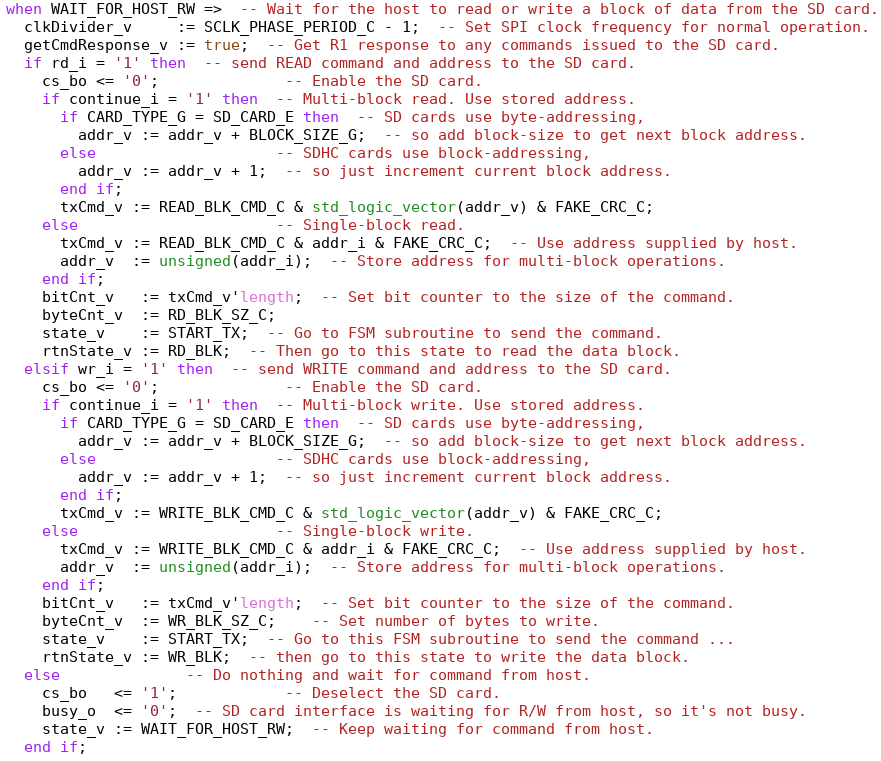
\includegraphics[width=\linewidth]{sdcardread}
  \caption{The SD card idle state code.}
  \label{fig:sdcardread}
\end{figure}

\begin{figure}
  \centering
  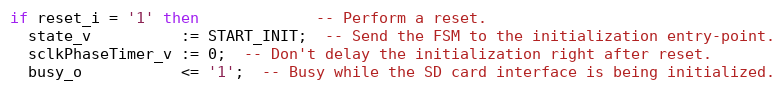
\includegraphics[width=\linewidth]{resetsdcard}
  \caption{The reset SD card code.}
  \label{fig:resetsdcard}
\end{figure}

\begin{figure}
  \centering
  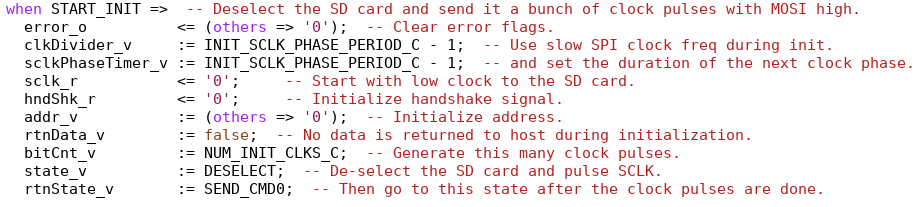
\includegraphics[width=\linewidth]{startsdcard}
  \caption{The SD card initial start up code.}
  \label{fig:startsdcard}
\end{figure}

\begin{figure}
  \centering
  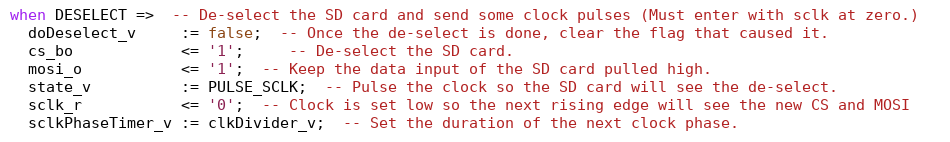
\includegraphics[width=\linewidth]{deselectsdcard}
  \caption{The deselect SD card code.}
  \label{fig:deselectsdcard}
\end{figure}

\begin{figure}
  \centering
  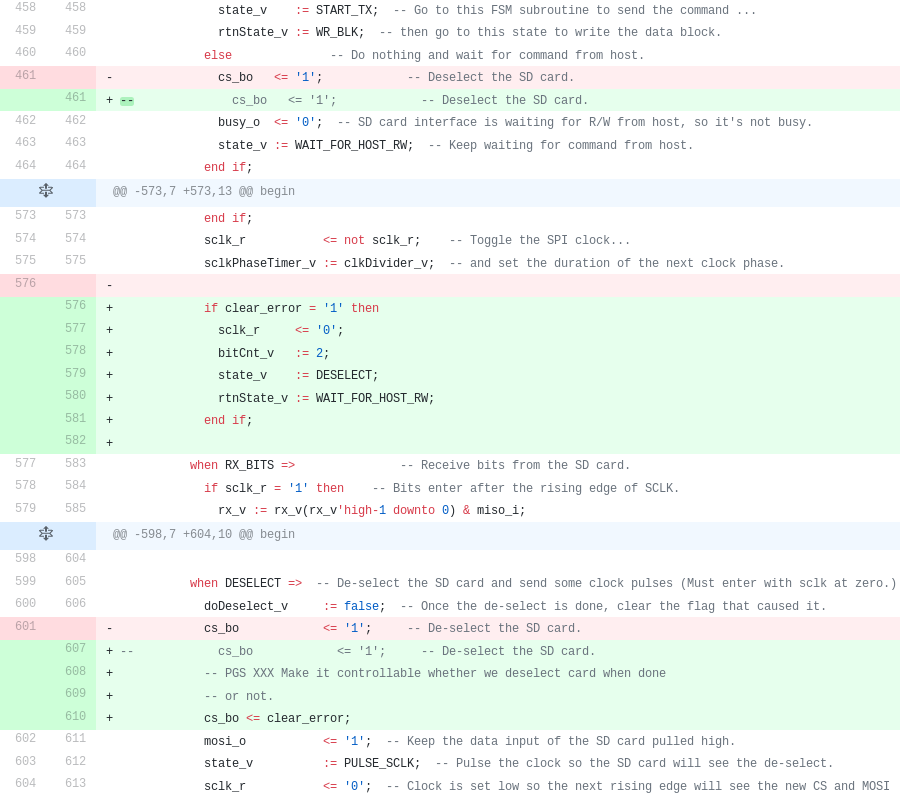
\includegraphics[width=\linewidth]{sdcardfix}
  \caption{The fixed read, write and idle code for the SD card controller..}
  \label{fig:sdcardfix}
\end{figure}

%----------------------------------------------------------------------------------------
%	SECTION 3
%----------------------------------------------------------------------------------------

\section{}

\label{Ch6 Sec3}

